\chapter{Related Work}
\label{ch:related_work}

This chapter provides a comprehensive analysis of previous research
and state-of-the-art technologies addressing multi-language static
code analysis, structural extraction, and name resolution. The
analysis is structured to evaluate the most recent and effective
techniques, critically examining their architectural choices,
underlying mechanisms, and current limitations. Understanding these
baseline approaches is essential for positioning the framework
proposed in this thesis, highlighting how it overcomes existing
bottlenecks in building language-agnostic dependency graphs.

The chapter is structured into five main sections: multi-language analysis
and tooling, language-agnostic syntactic representations,
graph models for reference resolution, direct precursor prototypes developed
within our research laboratory, and finally, the architectural positioning of
this thesis.

\section{Multi-Language Analysis and Tooling}
\label{sec:multilanguage_challenge}

Extracting structural and architectural information from source code requires
robust static analysis mechanisms. Traditionally, this process relies heavily on
\textbf{compiler front-ends}, such as Clang for C/C++ or Roslyn for
C\# \cite{lattner_llvm_2004}. A compiler front-end typically performs:
\begin{enumerate}
  \item \textbf{Lexical Analysis (Tokenization):} Converting text into a
    stream of tokens.
  \item \textbf{Syntactic Analysis (Parsing):} Grouping tokens into
    grammatical structures (syntax trees).
  \item \textbf{Semantic Analysis:} Type checking and symbol resolution.
\end{enumerate}

Because these tools must generate executable code, they possess a
mathematically sound and exhaustive understanding of the language's
semantics. However, this deep integration is also their primary
\textit{limitation}: they are inherently \textbf{coupled to a single
programming language}, its specific version, and its build ecosystem.

\subsection{Compiler Front-Ends and the $M \times N$ Problem}
\label{sec:compiler_frontends_mxn}

Developing a cross-language analysis system using language-specific
tools forces engineers to integrate various compiler
front-ends, each with its own output format, terminology,
and execution environment. If the system must support $M$ source
languages and $N$ analysis tools (or back-ends), each tool must be
individually integrated with each language's front-end, resulting in
$M \times N$ separate integration efforts. As both $M$ and $N$ grow,
this combinatorial complexity becomes unsustainable.

Modern compiler architectures, such as LLVM \cite{lattner_llvm_2004},
solve this problem by introducing an
\textbf{Intermediate Representation (IR)}: a standardized,
language-agnostic data structure that sits between the front-end
(which parses the source code) and the back-end (which performs
analysis or generates machine code). Each language requires only one
front-end that translates source code into the IR, and each tool
requires only one back-end that consumes the IR. The total number of
components is thus reduced from $M \times N$ to $M + N$. This
architectural transition is visually illustrated in Figure
\ref{fig:mxn_problem}.

\begin{figure}[htpb]
  \centering
  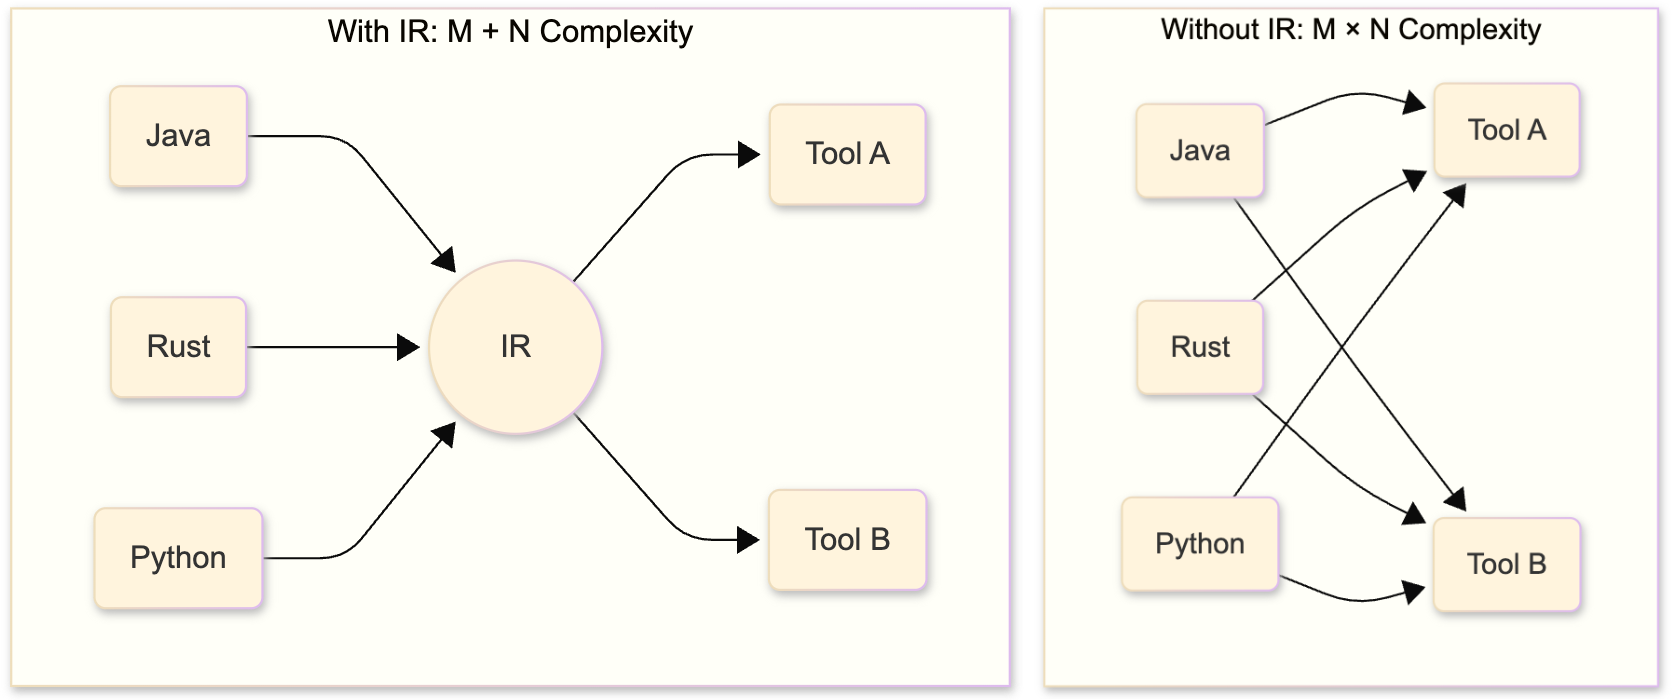
\includegraphics[width=\textwidth]{images/background/mxn_problem.png}
  \caption{Comparison between the $M \times N$ combinatorial
  explosion and the linear $M + N$ complexity achieved by introducing an IR.}
  \label{fig:mxn_problem}
\end{figure}

While LLVM uses a low-level IR focused on executable instructions,
architectural analysis requires a high-level, structural
representation. The same $M \times N$ decoupling principle applies to
this domain in two concrete ways:

\begin{itemize}
  \item \textbf{Internal decoupling:} Even within a single analysis
    tool, the pipeline contains multiple language-agnostic phases
    (name resolution, graph construction, export, visualization).
    Without an IR, each of these phases would need to handle the
    syntactic details of every supported language. With a shared IR,
    only the extraction phase is language-specific; all subsequent
    phases operate on a single, unified data model.
  \item \textbf{Ecosystem reuse:} A well-defined architectural IR can
    be consumed by multiple independent tools (e.g., architectural
    smell detectors, refactoring assistants, dependency auditors)
    without each tool reimplementing its own extraction logic for each
    language.
\end{itemize}

Designing a universal IR that captures the architectural semantics of
heterogeneous languages, without descending into low-level memory
layouts, is the core theoretical foundation required to build a truly
scalable, language-agnostic dependency extractor.

\subsection{Language Server Protocol (LSP)}
\label{sec:ir_and_lsp}

In recent years, protocols like the \textbf{Language Server Protocol
(LSP)} have attempted to standardize how development environments
interact with language-specific analyzers \cite{microsoft_lsp_spec}.
By standardizing the communication JSON-RPC interface, an IDE can
interact with any language server to request symbol definitions or
references. However, LSP is fundamentally designed for
\textbf{interactive, query-based use cases} (e.g., hovering over a
  variable to see its type, or requesting ``find references'' for a
specific symbol within an open file). Constructing a global
dependency graph of an entire repository requires a
\textbf{batch-processing approach}. Attempting to use LSP for this
purpose would involve artificially spoofing thousands of ``find
references'' queries across every symbol in every file, a process that
is highly stateful, incredibly slow, and simply suboptimal for
full-scale architectural extraction.

\subsection{Code Property Graph: Joern}
\label{sec:code_property_graphs}

Beyond interactive protocols like LSP, practical multi-language static
analysis often relies on frameworks that transform entire codebases into
queryable graph representations. In vulnerability discovery and security
research, this is typically achieved through fine-grained semantic graphs that
model instruction-level control and data flows across different programming
languages.

A well-known open-source platform in this domain is \textbf{Joern}
\cite{joern_docs}, originally developed by Yamaguchi et al. for
multi-language static analysis and vulnerability discovery
\cite{yamaguchi_modeling_2014}.

\textit{How it works:} Joern generates a \textit{Code Property Graph
(CPG)}, a data structure that unifies three representations: the AST, the
Control Flow Graph (CFG, which models statement execution order and conditional
branching), and the Program Dependence Graph (PDG, which tracks data and
control dependencies between operations) into a single, queryable graph
database. Analysts can query this graph using a specialized Scala-based Domain
Specific Language (Ocular/Joern dialect) to track data flow and identify
security flaws.

\textit{Weaknesses and Limitations:} Constructing a full Code Property Graph
incurs substantial computational overhead, as extracting CFGs and PDGs requires
modeling fine-grained runtime execution semantics. While this instruction-level
granularity is essential for vulnerability discovery, it is unnecessarily
heavy for high-level architectural analysis. Furthermore, Joern relies on
separate, heavyweight compiler front-ends (such as Eclipse JDT for Java or
Eclipse CDT for C/C++) rather than a unified parsing pipeline. As a result,
supporting additional languages requires integrating dedicated compiler tools,
reproducing the front-end coupling of the $M \times N$ problem.

\subsection{Architectural Analyzers: Arcan and Depends}
\label{sec:architectural_dependency_analyzers}

While platforms like Joern operate at the instruction level, architectural
analysis works at a higher level, extracting component and dependency graphs to
evaluate structural health, modularity, and technical debt. Two widely used
tools in this domain, which also serve as experimental baselines in this
thesis, are \textbf{Arcan} and \textbf{Depends}.

\textbf{Arcan} \cite{fontana_arcan_2017} is a static analysis
tool developed by Fontana et al. dedicated to the automatic detection of
architectural smells and the monitoring of architectural decay across software
releases \cite{sas_investigating_2019}. Similar component and
dependency graphs are used in industrial architectural suites (such as
SonarQube or Structure101) to monitor modularity, but Arcan uniquely formalizes
the automated detection of architectural smells and architectural
technical debt.

\textit{How it works:} Arcan analyzes software projects (primarily Java and
C/C++) by extracting multi-layered dependency graphs that capture structural
relations among packages, classes, and methods. On top of these graphs, Arcan
executes graph-based algorithms and computes structural and topological metrics
to detect critical dependency smells, such as Cyclic Dependency, Hub-Like
Dependency, and Unstable Dependency. Furthermore, it tracks the introduction,
persistence, and refactoring of these smells over commit histories and release
cycles, providing quantifiable indicators of architectural technical debt.

\textit{Role and Relevance to this Work:} Within our research laboratory,
Arcan represents the primary reference baseline for architectural analysis;
both precursor prototypes to this thesis, Skullian \cite{refolli_2023} and
Entangle \cite{teruzzi_2024}, evaluated their dependency extraction accuracy
and graph similarity against Arcan's output. However, Arcan's extraction
pipeline relies on language-specific frontends and bytecode analyzers (such as
Spoon for Java or compiler-based parsers for C/C++). Adding support for emerging
or polyglot software systems (e.g., in Rust, Python, or Go) requires
engineering dedicated frontends tailored to each language's compiler ecosystem.
This limitation directly motivates the research in this thesis: designing a
lightweight, uniform, and language-agnostic extraction engine capable of
producing faithful dependency graphs across heterogeneous languages, serving as
an effective frontend for architectural analysis tools like Arcan.

\textbf{Depends} \cite{depends_github} is an open-source, multi-language static
analysis framework specifically designed to extract fine-grained syntactical
dependencies among code entities (files, types, and methods). Developed to
support architecture recovery, code visualization, and modularity evaluation,

\textit{How it works:} Depends relies on language-specific parsers generated
via \textbf{ANTLR} grammars. For each supported language, an ANTLR-generated
parser constructs an Abstract Syntax Tree (AST), which is subsequently visited
to infer explicit syntactic relationships such as inheritance (\texttt{extend},
\texttt{implement}), behavioral interactions (\texttt{call}, \texttt{create}),
type declarations (\texttt{parameter}, \texttt{return}), and imports. The
extracted dependencies are then aggregated into a unified dependency matrix and
exported into standard interchange formats, such as JSON or Graphviz DOT.

\textit{Role and Relevance to this Work:} In this thesis, Depends represents a
crucial state-of-the-art multi-language reference baseline. Alongside Arcan,
Depends is directly utilized in Chapter \ref{ch:evaluation_results} to benchmark
and validate the accuracy, graph similarity, and extraction performance of
Omnideps across heterogeneous, multi-language codebases.

\textit{Weaknesses and Limitations:} Although Depends successfully supports
multiple programming languages, its reliance on language-specific ANTLR
grammars presents some practical limitations:
\begin{itemize}
  \item \textbf{Grammar Maintenance Burden:} While both tools require
    language-specific logic to recognize initial code constructs, Depends
    authors and maintains independent ANTLR grammars (\texttt{.g4}) for each
    supported language. In contrast, our pipeline leverages existing,
    widely adopted Tree-sitter grammars and strictly isolates language-specific
    parsing to Phase 1, converting the syntax tree into a shared intermediate
    model before any resolution begins.
  \item \textbf{Parsing Algorithm Characteristics:} ANTLR utilizes a
    top-down $LL(*)$ parsing strategy, which can incur non-trivial
    memory and execution overhead on large source files compared to
    bottom-up GLR parsing algorithms. Conversely, Tree-sitter
    utilizes a bottom-up GLR parser implemented in native C that is
    inherently error-tolerant, producing a usable syntax tree even
    from malformed or incomplete source files.
  \item \textbf{Lack of a Formal Unified IR and Scope Model:} Depends maps
    AST nodes directly to dependency records without an intermediate, formal
    algebraic representation. As a result, name resolution and expression
    handling are implemented through ad-hoc logic within each language's AST
    visitor, rather than through a single, unified resolution engine. In
    contrast, our pipeline evaluates reference queries through a formal
    query algebra over a language-agnostic Scope Tree, ensuring consistent
    and mathematically defined resolution semantics across all supported
    languages.
\end{itemize}

\section{Language-Agnostic Syntax Representations}
\label{sec:language_agnostic_syntax}

A major challenge in cross-language static analysis is the profound
heterogeneity of the Abstract Syntax Trees (ASTs) generated by
different parsers.  Analyzing multi-language software with a single
unified backend therefore requires a common level of abstraction. In
the literature, prior research has largely pursued this goal at the
syntactic level by normalizing source code from different programming
languages into unified tree representations, such as intermediate XML
markup or universal abstract syntax trees.

\subsection{Syntactic Wrapping: srcML}

\textbf{srcML} \cite{collard_srcml_2016} is an infrastructure and
XML-based format designed to represent source code by wrapping the
original raw text with syntactic XML tags.

\textit{How it works:} Instead of transforming code into an abstract
data structure that discards formatting, srcML parses the code and
produces an XML document that preserves the exact original text,
including whitespace and comments. It overlays this text with
syntactic boundaries (e.g., \texttt{<class>}, \texttt{<function>},
\texttt{<expr>}). Analysts can then use standard XML querying tools,
such as XPath, to extract facts and relationships from the codebase.

For example, given the simple C++ snippet in Listing
\ref{lst:srcml_cpp}, srcML translates it into the XML format shown in
Listing \ref{lst:srcml_xml}, preserving the original tokens while
exposing the syntax tree structure \cite{srcml_about}.

\begin{lstlisting}[language=C++,caption={Example of a simple C++ function to be analyzed by srcML.},label={lst:srcml_cpp}]
#include "rotate.h"

// rotate three values
void rotate(int& n1, int& n2, int& n3) {
  // copy original values
  int tn1 = n1, tn2 = n2, tn3 = n3;

  // move
  n1 = tn3;
  n2 = tn1;
  n3 = tn2;
}
\end{lstlisting}

\begin{lstlisting}[basicstyle=\ttfamily\footnotesize, language=XML,caption={The resulting srcML representation, keeping formatting intact but injecting syntactic tags.},label={lst:srcml_xml}]
<cpp:include>#<cpp:directive>include</cpp:directive> <cpp:file>"rotate.h"</cpp:file></cpp:include>

<comment type="line">// rotate three values</comment>
<function><type><name>void</name></type> <name>rotate</name><parameter_list>(<parameter><decl><type><name>int</name><modifier>&amp;</modifier></type> <name>n1</name></decl></parameter>, <parameter><decl><type><name>int</name><modifier>&amp;</modifier></type> <name>n2</name></decl></parameter>, <parameter><decl><type><name>int</name><modifier>&amp;</modifier></type> <name>n3</name></decl></parameter>)</parameter_list> <block>{<block_content>

  <comment type="line">// copy original values</comment>
  <decl_stmt><decl><type><name>int</name></type> <name>tn1</name> <init>= <expr><name>n1</name></expr></init></decl>, <decl><type ref="prev" /><name>tn2</name> <init>= <expr><name>n2</name></expr></init></decl>, <decl><type ref="prev" /><name>tn3</name> <init>= <expr><name>n3</name></expr></init></decl>;</decl_stmt>

  <comment type="line">// move</comment>
  <expr_stmt><expr><name>n1</name> <operator>=</operator> <name>tn3</name></expr>;</expr_stmt>
  <expr_stmt><expr><name>n2</name> <operator>=</operator> <name>tn1</name></expr>;</expr_stmt>
  <expr_stmt><expr><name>n3</name> <operator>=</operator> <name>tn2</name></expr>;</expr_stmt>
</block_content>}</block></function>
\end{lstlisting}

\textit{Weaknesses and Limitations:} While srcML is highly robust for
lightweight fact extraction and refactoring tasks, it is essentially
a syntactic markup rather than a semantic model. It does not provide
built-in name resolution or cross-file dependency linking; it simply
unifies the syntax. Furthermore, its parser ecosystem is currently
restricted to a limited set of languages (C, C++, C\#, and Java), and
it does not support the full range of available programming languages,
limiting the future extensibility of the analysis framework.

\textit{Relevance:} \textit{Relevance:} While srcML cannot be adopted
in this work due to its current language restrictions, its underlying
philosophy remains highly relevant. By mapping syntactic constructs
to a common vocabulary of structural annotations across all supported
languages, it provides a unified baseline for core program elements.
Adopting such a cross-language unified annotation scheme could
represent an interesting alternative for the extraction layer,
significantly reducing the need for complex heuristics to recognize
corresponding constructs across different parsing trees.

\subsection{Universal ASTs: Babelfish}

A widely explored direction in multi-language analysis is
transforming source code into a unified, language-agnostic tree
representation. A pioneer in this domain was \textbf{Babelfish}
\cite{babelfish_uast}, an open-source framework that introduced the
concept of the \textit{Universal Abstract Syntax Tree (UAST)}.
Babelfish aimed to parse any programming language into a standardized
syntax tree annotated with language-independent semantic roles. In a
similar vein, recent research by Curtis
\cite{curtis_language-agnostic_2022} and Schiewe et al.
\cite{schiewe_advancing_2022} focuses on generating language-agnostic
ASTs to analyze heterogeneous, cloud-native microservices. In
distributed systems, microservices frequently employ different
programming languages, making traditional single-language analyzers
insufficient for tracing cross-service architectural dependencies
(e.g., a Python service invoking a Java endpoint).

\textit{How it works:} To bridge language differences, these approaches
introduce an explicit multi-stage translation pipeline. Language-specific
parsers or drivers (often wrapping Tree-sitter or native compiler frontends)
first produce language-dependent ASTs. Next, dedicated transformation drivers
map syntax nodes into a serialized, language-agnostic representation, either an
annotated UAST with normalized node types or a standardized intermediate format
(frequently serialized in JSON or protocol buffers). Finally, generic component
analyzers traverse this normalized tree to extract architectural abstractions
(such as endpoints, controllers, and data models) regardless of the source
language.

\textit{Weaknesses and Limitations:} Although effective for coarse-grained
syntactic classification, relying on a Universal AST presents several major
limitations for deep architectural analysis. First, maintaining dedicated
transformation drivers is costly: every supported grammar requires continuous
manual engineering to map evolving language syntax into the universal schema.
Second, full-tree normalization incurs significant computational and memory
overhead, as entire codebases must be translated into statement-level and
expression-level universal syntax trees, capturing low-level details (such as
arithmetic operations or loop constructs) that are irrelevant for architectural
dependencies. Third, attempting to unify diverse language syntaxes into a single
syntactic tree is inherently lossy: collapsing language-specific constructs
into generic node kinds discards the distinct scoping and visibility
semantics required for faithful name resolution.

\textit{Relevance:} Our work directly addresses these drawbacks by avoiding an
instruction-level Universal AST entirely. Instead of normalizing all source
syntax into a single monolithic tree, we perform selective, heuristic-based
extraction directly on Tree-sitter Concrete Syntax Trees (CSTs). We extract
only high-level architectural constructs (modules, types, signatures, and
reference queries) into a lightweight Intermediate Representation
($\mathcal{D}_{IR}$), discarding intra-procedural statement syntax immediately
after extraction. Crucially, rather than forcing heterogeneous scoping rules
into a generic syntactic schema, our pipeline preserves language-specific
resolution semantics through the declarative configuration $\mathcal{K}$
evaluated during Phase 2.

\section{Graph Models for Reference Resolution}
\label{sec:graph_models_reference_resolution}

Once the structural components of a codebase are identified, the
subsequent challenge is resolving identifiers (e.g., variable usages,
method calls, and type references) to their concrete definitions across complex,
nested scopes. This section evaluates declarative and automaton-based graph
models developed in the literature for reference resolution.

\subsection{Path-Based Resolution: Scope Graphs}
\label{sec:scope_graphs}

\textbf{Scope Graphs} \cite{zwaan_scope_2023}, developed by
researchers at TU Delft, provide a foundational, language-parametric
theoretical framework for name binding and resolution.

\textit{How it works:} The model abstracts away the AST entirely,
representing the program's lexical structure as a graph. Lexical
scopes are represented as nodes, and visibility or reachability rules
(such as lexical nesting or module imports) are represented as
directed edges. Resolving a name becomes a formal path-finding
problem within this graph, governed by specific regular expressions
that dictate valid resolution paths.

\textit{Weaknesses and Limitations:} The main weakness of standard
Scope Graphs is their lack of scalability. The model typically
requires a whole-program analysis, meaning the entire project must be
parsed and translated into a single, massive graph in memory before
resolution can begin. They struggle with incremental updates, making
them computationally prohibitive for very large codebases.

\subsection{Pushdown Navigation: Stack Graphs}
\label{sec:stack_graphs}

\textbf{Stack Graphs} \cite{creager_stack_2023} are the direct
successor to Scope Graphs, developed and heavily utilized by GitHub
to provide code navigation (e.g., "jump to definition") at an industrial scale.

\textit{How it works:} They extend Scope Graphs by introducing a
"Symbol Stack" and two new node types: \textit{push} and \textit{pop}
nodes. This crucial addition allows the graph to be built
incrementally, file by file. When a reference is queried, the
algorithm walks the graph, pushing identifiers onto the stack at
\textit{push} nodes and popping them at \textit{pop} nodes. A path is
considered valid, and the reference resolved, if the symbol stack is
completely empty when a definition node is reached.

\textit{Weaknesses and Limitations:} While theoretically elegant and
excellent for localized IDE queries, Stack Graphs possess significant
practical limitations when repurposed for total dependency
extraction. First, constructing a Stack Graph requires the creation
of highly complex and verbose grammars (using the Tree-sitter Graph
or TSG language) for every single language. Second, because
resolution in Stack Graphs relies on a pushdown automaton traversing
graph edges, finding all dependencies requires executing this
graph-walking algorithm from every single reference. In highly
interconnected codebases with deep import chains, this mechanism
suffers from a \textit{path-explosion} problem: the algorithm
evaluates thousands of combinatorial paths simultaneously to verify
stack emptiness, leading to severe memory and performance
bottlenecks. Conversely, our approach avoids this combinatorial
explosion by replacing unguided graph traversal with deterministic
algebraic lookups on a Scope Tree.

\section{Direct Precursors}
\label{sec:precursors}

This thesis represents the culmination and third iteration of a
continuous research effort initiated by Francesco Refolli and later
advanced by Luca Teruzzi, building upon two previous prototypes
which laid the critical foundation for the current solution.

\subsection{Stack-Graph Resolution: Skullian}
\label{sec:skullian}

\textbf{Skullian} \cite{refolli_2023} was the initial prototype of
this research line, developed by Dr. Francesco Refolli (who currently
serves as co-advisor for this thesis). It attempted purely
language-agnostic dependency extraction by combining Tree-sitter for
parsing with Stack Graphs for name resolution.

\textit{How it works:} It parsed the source code with Tree-sitter and
used custom TSG rules to map the generated CST into a Stack Graph. It
then used the built-in Stack Graph path-finding algorithm to resolve
all references and build a dependency graph.

\textit{Weaknesses and Limitations:} The evaluation of Skullian
exposed practical and scalability limits of Stack Graphs for
architectural-level dependency extraction.
\begin{itemize}
  \item \textbf{Grammar Complexity}: Writing the language-specific
    TSG rules were highly verbose and complex, requiring thousands of
    lines of configuration for a single language like Java. This made
    the system difficult to maintain and extend.
  \item \textbf{Path Explosion and Cycle Detection Issues}: The Stack
    Graph size grew very big even for modest projects, causing
    reference resolution times to scale exponentially. To avoid
    infinite loops, the system relied on a cycle-detection heuristic.
    However, in real-world software, this heuristic frequently cut
    off valid resolution paths passing through the root node, leading
    to missed dependencies. Relaxing the path-similarity constraints
    (MAX\_SIMILAR\_PATH\_COUNT) inevitably resulted in system stalls or
    Out-Of-Memory (OOM) crashes, making large-scale projects unanalyzable.
\end{itemize}

\subsection{Scope-Climbing Resolution: Entangle}
\label{sec:entangle}

\textbf{Entangle} \cite{teruzzi_2024} represents the second iteration
of this research line, developed by Luca Teruzzi with the explicit
goal of overcoming the critical performance and memory scalability
barriers encountered by Skullian.

\textit{How it works:} To achieve this, Entangle completely abandoned
Stack Graphs, introducing a custom, highly efficient two-phase name
resolution model.
\begin{itemize}
  \item In the first phase, it performs a static traversal of the
    source code's CST (generated via Tree-sitter) to reconstruct a
    hierarchical \textbf{Component Graph} representing packages,
    classes, and methods, while storing unresolved references as
    nested, unresolved dependency queries (modeled via recursive
    QueryData structures). A stack-based symbol table is maintained
    during this phase to map local variables to their respective types.
  \item \textbf{Phase Two: Scope Climbing Resolution}: In the second
    phase, the engine resolves these queries directly on the
    component graph using a custom \texttt{Lookup and Lookdown}
    algorithm. The lookup step ascends the component hierarchy to
    resolve the root of the query (handling imports as direct
    architectural bridges), while the lookdown step descends through
    the target component's children and inheritance chains to resolve
    nested members (e.g., method calls and field accesses).
\end{itemize}

To remain strictly language-agnostic, Entangle relies on a
configuration \textbf{dispatch table} for each supported language.
Users explicitly map abstract architectural concepts (e.g. Class,
Method) to the concrete CST node identifiers defined by that
language's Tree-sitter grammar (e.g., class\_declaration or
function\_item), isolating language-specific differences in a
declarative configuration layer

\textit{Weaknesses and Limitations:} Despite drastically improving
performance, outperforming Arcan \cite{fontana_arcan_2017} by completing
analyses in approximately half the execution time on average,
Entangle still exhibits structural and functional limitations:

\begin{itemize}
  \item \textbf{Manual Dispatch Table Configuration}: The dispatch
    table requires manual configuration for each language, demanding
    deep knowledge of the specific Tree-sitter grammar and its node
    identifiers.
  \item \textbf{Lack of Formalization}: Entangle's internal model
    lacks a rigorous mathematical formalization, which can lead to
    inconsistencies in name resolution and dependency extraction.
  \item \textbf{No Support for Generics}: The prototype completely
    lacks the ability to resolve and propagate parameterized types
    (Generics), resulting in a notable accuracy loss on
    template-heavy codebases.
  \item \textbf{Monolithic Module Resolution}: The framework is
    currently unable to partition distinct package modules (such as
    multiple Rust crates) within a single analyzed directory, causing
    them to collapse into a single dependency tree and compromising
    namespace isolation.
\end{itemize}

\section{Positioning of the Proposed Work}

The framework presented in this thesis directly addresses the
limitations of both the broad state-of-the-art technologies and the
specific precursor prototypes.

By relying strictly on Tree-sitter and its cursor navigation, we
maintain a lightweight, single-frontend extraction process, avoiding
the heavy, language-specific pipelines and CFG computational overhead
of tools like Joern. Unlike Arcan, which requires dedicated compiler-based
frontends (such as Spoon) for each supported language, and unlike Depends,
which demands maintaining independent ANTLR grammars and visitor passes,
Omnideps overcomes the $M \times N$ problem through cross-grammar structural
convergence on Concrete Syntax Trees. Instead of facing the severe
scalability issues of Stack Graphs (as evidenced by Skullian), or resorting
to lossy Universal AST translations (as seen in Curtis and Schiewe), we have
formalized a robust Intermediate Representation ($\mathcal{D}_{IR}$) based on
algebraic data types.

Crucially, compared to Entangle, we have completely eliminated the
need for a manual "dispatch table". Instead, our framework implements
a \textbf{Heuristic-based extraction}. Because Tree-sitter parsers
use highly predictable naming conventions across different grammars
(e.g., node names consistently containing \texttt{struct},
\texttt{class}, \texttt{function}, or \texttt{module}), we extract
constructs by applying heuristics directly on the original CST.
Coupled with a feature-based configuration to manage broad behavioral
differences (like identifying if a language uses directory-based
packages or inline modules), this makes the extraction phase natively
language-agnostic.

The formal IR natively models complex,
multi-layered module hierarchies (solving the namespace collision
issues). The resolution engine has been rigorously expanded to
support generic types, evaluated access paths, and accurate type
bounds. Ultimately, this thesis elevates the experimental concepts of
previous iterations into a mathematically sound, provably decoupled
language-agnostic architectural analyzer.
